% This is samplepaper.tex, a sample chapter demonstrating the
% LLNCS macro package for Springer Computer Science proceedings;
% Version 2.21 of 2022/01/12
%
\documentclass[runningheads]{llncs}
%
\usepackage[T1]{fontenc}
% T1 fonts will be used to generate the final print and online PDFs,
% so please use T1 fonts in your manuscript whenever possible.
% Other font encondings may result in incorrect characters.
%
\usepackage{graphicx}
% Used for displaying a sample figure. If possible, figure files should
% be included in EPS format.
%
% If you use the hyperref package, please uncomment the following two lines
% to display URLs in blue roman font according to Springer's eBook style:
%\usepackage{color}
%\renewcommand\UrlFont{\color{blue}\rmfamily}
%\urlstyle{rm}
\usepackage{hyperref}
\usepackage[acronym]{glossaries}
\glsdisablehyper
\usepackage{todonotes}
\usepackage{subcaption}
\usepackage{caption}
\captionsetup[table]{name=Tab.}
\usepackage{xspace}
\usepackage{siunitx}
\usepackage{multicol}
\usepackage{multirow}
\usepackage{booktabs}
\usepackage{svg}
\usepackage{xurl}
\usepackage[sort,compress]{cite}

% \usepackage{draftwatermark}
% \SetWatermarkText{DRAFT}
% \SetWatermarkScale{5}
% \usepackage{framed}

% I inserted this since I always got a numbered but blank first page
% I do not know why
% I followed this advise: https://tex.stackexchange.com/a/434340
\usepackage{atbegshi}
\AtBeginDocument{\AtBeginShipoutNext{\AtBeginShipoutDiscard}\addtocounter{page}{-1}}



\newcommand{\citeurl}[1]{\unskip\footnote{{\scriptsize \url{#1}}}}
\newcommand{\pkgname}[1]{{\scriptsize \textsf{#1}}}
\newcommand{\projname}[1]{{\small \textsf{#1}}}
% \newcommand{\toolname}[1]{{\scriptsize \texttt{#1}}}
\newcommand{\toolname}[1]{{\small \texttt{#1}}}

\newcommand{\python}{\projname{Python}\xspace}
\newcommand{\cp}{\projname{CPython}\xspace}
\newcommand{\cpv}[1]{\projname{CPython 3.{#1}}\xspace}
\newcommand{\flask}{\projname{Flask}\xspace}
\newcommand{\django}{\projname{Django}\xspace}
\newcommand{\rust}{\projname{Rust}\xspace}
\newcommand{\java}{\projname{Java}\xspace}
\newcommand{\cc}{\projname{C\nolinebreak\hspace{-.05em}\raisebox{.4ex}{\tiny +}\nolinebreak\hspace{-.10em}\raisebox{.4ex}{\tiny +}}\xspace}

\renewcommand{\tableautorefname}{Tab.}
\renewcommand{\figureautorefname}{Fig.}
\renewcommand{\sectionautorefname}{Sec.}
\renewcommand{\subsectionautorefname}{Sec.}
\renewcommand{\subsubsectionautorefname}{Sec.}

\newacronym{pep}{PEP}{Python Enhancement Proposal}
\newacronym{watt}{W}{Watt}
\newacronym{joule}{J}{Joule}
\newacronym{sut}{SUT}{System Under Test}
\newacronym{pypi}{PyPI}{Python Packaging Index}
\newacronym{pyperformance}{\projname{pyperformance}}{The Python Performance Benchmark Suite}
\newacronym{os}{OS}{Operating System}
\newacronym{cpu}{CPU}{Central Processing Unit}
\newacronym{rpi}{RPI}{Raspberry Pi}
\newacronym{rapl}{RAPL}{Running Average Power Limit}


\newcommand{\rpi}[1]{\toolname{Raspberri Pi #1}\xspace}
\newcommand{\rpia}{\gls{rpi}\xspace}

%
% Page limit: 12 to 16 pages
\begin{document}
%
\title{Energy Consumption of Python Performance Benchmarks Depends on Execution Environments}
%
%\titlerunning{Abbreviated paper title}
% If the paper title is too long for the running head, you can set
% an abbreviated paper title here
%
\author{Oskar Emil Breindahl\inst{1}
\and
Rolf-Helge Pfeiffer\inst{1}\orcidID{0000-0003-2585-6473}
%\and
%Third Author\inst{3}\orcidID{2222--3333-4444-5555}
}
%
\authorrunning{O. Breindahl, R.-H. Pfeiffer}\
%\authorrunning{Fst. Author}\
% First names are abbreviated in the running head.
% If there are more than two authors, 'et al.' is used.
%
\institute{IT University of Copenhagen, Rued Langgaards Vej 7, 2300 Copenhagen
\email{\{osbr,ropf\}@itu.dk}}
% \institute{A University, Street, City
% \email{author@university.edu}}
%\url{http://www.springer.com/gp/computer-science/lncs} \and
%ABC Institute, Rupert-Karls-University Heidelberg, Heidelberg, Germany\\
%\email{\{abc,lncs\}@uni-heidelberg.de}}
%
\maketitle              % typeset the header of the contribution
%
\begin{abstract}
% The abstract should briefly summarize the contents of the paper in 150--250 words.
\python is one of the most used programming languages in the world.
Developers of the \python interpreter increase its performance over recent releases and measure these with \gls{pyperformance}.
However, little is known about the impact of performance increases on the energy consumption of \python programs when executed in different environments like operating systems or processors.
In this paper, we study via a controlled lab experiment the energy consumption of benchmarks from \gls{pyperformance} when executed on five versions of the \python interpreter \cp, on four different operating systems, and on two different processors.
Our results indicate that executing Python programs on a Cortex-A72 processor running Manjaro Linux and \cpv{12} is XX times more energy efficient than on a Cortex-A53 running FreeBSD with \cpv{10}.
Even on the same processor, energy consumption of \python programs decreases by up to XX\% when executed on Manjaro Linux and a newer versions of \python, compared to other operating systems and older versions of \cp.
\keywords{Software engineering \and Energy consumption \and CPython.}
\end{abstract}

\section{Introduction}\label{sec:introduction}

The responsibility of software developers to create sustainable and energy-efficient software is becoming more and more apparent\cite{caballar2024we} and the environmental impact and sustainability of software is increasingly studied.\cite{ahmad2023green,caballar2024we,freed2023investigation,gupta2021chasing,adersma2022green,lamprakos_energy,holm2020gpu,reya2023greenpy,lorincz2019greener,freed2023investigation,roque2025unveiling,paul2023comprehensive,ahmad2023green,tiwari2021review}\todo{Too much sausage?}.

\python is likely the most popular~\cite{djurdjev2024popularity,pypl,tiobe} and most used~\cite{stackover, statista} programming language in the world.
Big corporations create software products with it.
For example, Google’s \projname{YouTube} is powered by \python~\cite{winters2020software}, circa 20\% of \projname{Facebook}’s infrastructure is written in \python~\cite{komorn2016python}, \projname{Instagram} is a \python application~\cite{ni2016web}, or circa 80\% of \projname{Spotify}’s backend services are written in \python~\cite{van2013how}.

Like other dynamically typed and interpreted programming languages, running certain \python programs is reported to be slow and of low energy efficiency~\cite{pereira_rank_efficiency}.
In recent years, the developers of \cp, the reference implementation of the \python interpreter, continuously increase the performance of \cp, i.e., they increase execution times of \python programs.

Since energy consumption of software is influenced by execution times ($E = P \times t$) and since \python is a comparably slow dynamically typed interpreted language, it might be worthwhile to continue to increase performance of \cp over the coming releases.
We believe that additionally focusing on the energy consumption of programs executed on \cp should be in focus as well.\todo{Improve this.}
Currently, there is no \gls{pep} to reduce energy consumption of \python programs as there are \glspl{pep} to increase performance of \cp~\cite{pep_index}.

In this paper, we present a light weight experiment design that allows to compare the energy consumption of \python programs that are executed on various configurations of hardware, \gls{os}, and \python versions.
Our goals are \emph{a)} to investigate if certain configurations of \glspl{cpu}, \glspl{os}, and \python versions significantly impact the energy consumption of \python benchmarks from \gls{pyperformance}, and \emph{b)} to provide an experiment design that is so light weight that \cp developers can efficiently include it in their current setup when running \gls{pyperformance}.

We investigate the following three research questions:
\begin{itemize}
  \item \textbf{RQ1:} \textit{How do different \glspl{cpu} impact the energy consumption of \gls{pyperformance} benchmarks?}
  \item \textbf{RQ2:} \textit{How do different \glspl{os} impact the energy consumption of \gls{pyperformance} benchmarks?}
  \item \textbf{RQ3:} \textit{How do different versions of \cp impact the energy consumption of \gls{pyperformance} benchmarks?}
\end{itemize}

We measure energy consumption of a \gls{sut} with an \toolname{Otii Ace Pro}~\cite{qoitech2022otii}.
In this paper, \glspl{sut} are a \toolname{Raspberry Pi 3B+} (ARM-Cortex-A53) and \toolname{Raspberry Pi 4B} (ARM-Cortex A72) respectively.
% TODO: Add these to references
% https://datasheets.raspberrypi.com/rpi3/raspberry-pi-3-b-plus-product-brief.pdf
% https://datasheets.raspberrypi.com/rpi4/raspberry-pi-4-datasheet.pdf
On each \toolname{Raspberry Pi}, we sequentially deploy one of the four Unix(-like) \glspl{os} \projname{Alpine}, \projname{Manjaro}, \projname{Ubuntu}, and \projname{FreeBSD}.
On each \gls{os}, we sequentially deploy different versions of \cp.
The combination of \gls{cpu}, \gls{os}, and version of \cp is a configuration.
In our experiment, we investigate 40 different configurations.
For each configuration, we execute \gls{pyperformance} and measure execution times of various benchmarks and their power draw during execution.

We find that all three variables of \gls{cpu}, \gls{os}, and version of \cp have a statistically significant impact on energy consumption during benchmark execution.
% Fill in high level results here!


The contributions of this paper are:
\begin{itemize}
  \item We present an experiment design to directly measure the energy consumption of 40 different configurations of \gls{cpu}, \gls{os}, and version of \cp.
  \item We demonstrate that benchmarks executed on certain configurations of \gls{cpu}, \gls{os}, and version of \cp consume significantly less energy compared to other widely used configurations.
  \item We provide a replication kit\footnote{\url{https://github.com/oskarbreindahl/Python_Application_Energy_Consumption}} that allows to automatically replicate our results. It also contains all results reported in this paper and allows for reproduction.\todo{Move repo and anonymize link for review.}
\end{itemize}

\section{Background \& Terminology}\label{sec:background}

\noindent\textbf{System Under Test:} \emph{Raspberry Pis} are credit card sized ARM-based single-board computers produced by the Raspberry Pi Foundation\cite{raspberry_pi_website}.
These inexpensive computers are often used in lab experiments, e.g., \cite{zhao2015exploring,pfeiffer2024energy}.\todo{Check if the former can be used for that statement.}
We use two versions of \toolname{Raspberry Pis} as \glspl{sut} for the research in this paper.
First, the \toolname{Raspberry Pi 3B+} with a four core ARM-Cortex-A53 \gls{cpu} and 1GB RAM and second, the \toolname{Raspberry Pi 4B} with a four core ARM-Cortex A72 \gls{cpu} and XXGB RAM\todo{Which version did you use?}.
Both processors are 64-bit running at 1.4GHz and 1.8GHz respectively.
The main difference between the Cortex-A53 and A72 architecture is that the latter supports out-of-order memory operations.

\noindent\textbf{Operating Systems:} We execute our experiment on four \glspl{os}.
One Unix, \projname{FreeBSD}\cite{freebsd_website}, and the three Linux distributions \projname{Alpine}\cite{alpine_website}, \projname{Manjaro}\cite{manjaro_website}, and \projname{Ubuntu}\cite{ubuntu_website}.\todo{Add precise versions+kernel and libc versions}
In the Linux realm, \emph{distributions} are a collection of \gls{os} kernel, init system, tools, and applications, which in the case of Unixes like \projname{FreeBSD} are all provided together as a single system.
For example, \projname{Ubuntu} is a \projname{Debian}-based distribution (relying on \projname{systemd} and the \projname{apt} package manager) that focuses on stability and \projname{Manjaro} is based on \projname{Arch Linux} (relying on \projname{systemd} and the \projname{pacman} package manager) with a rolling-release update model.
\projname{Alpine Linux} differs from the other two Linuxes in the choice of basic software.
It relies on \projname{musl} instead of \projname{glibc} as C standard library, \projname{BusyBox} instead of \projname{GNU Core Utilities}, and \projname{OpenRC} as init system instead of \projname{systemd}.
\todo{Add sentence on popularity and widely used on servers/containers}

\noindent\textbf{Python:} is likely the most popular~\cite{djurdjev2024popularity,pypl,tiobe} and most used~\cite{stackover, statista} programming language in the world.
There are many different implementations of the language, e.g., the reference implementation \cp, \projname{pypy}, \projname{MicroPython}, etc.
In this paper we consider the --at the time of writing-- latest releases of the five supported versions of \cp: \cpv{9.22}, \cpv{10.17}, \cpv{11.12}, \cpv{12.10}, and \cpv{13.3}.
In the remainder, we denote these versions by their major and minor version number, e.g., \cpv{9}, \cpv{10}, etc.

\noindent\textbf{\acrlong{pyperformance}:} is an open-source benchmarking tool~\cite{pyperf_git} that \cp developers use to report performance improvements of new versions of \cp, see e.g., the release notes for \cpv{12}~\cite{py312}.
\gls{pyperformance} consists of 87 benchmark programs that are organized in seven \emph{groups}.
For our experiment, we select three \textit{``'High-level' applicative benchmarks''}\cite{pyperf_docs} benchmarks from the \toolname{apps} group: \toolname{2to3}, \toolname{tornado\_http} and \toolname{chameleon}.


\noindent\textbf{Measuring Energy Consumption:} There are two main ways to measure the energy consumption of a \gls{sut}.
On certain Intel-based processors, one could use \gls{rapl}~\cite{khan2018rapl}, which is a built-in \gls{cpu} feature that allows --amongst others-- to estimate power draw of running programs.
% https://greencompute.uk/Measurement/RAPL
Since this feature is not available on a broad range of \glspl{cpu}, e.g., the ARM-Cortex architectures in our experiment, one can always directly measure power draw of a \gls{sut} with a suitable power meter~\cite{kavanagh2019rapid}.
In our experiment, we use the \toolname{Otii Ace Pro}~\cite{otii_website,qoitech2022otii}, which is a power supply with combined scriptable power-meter.
We use it to record \emph{power draw} ($P$ in Watts [W]) and execution times of benchmarks (in seconds [s])
We compute \emph{energy consumption} ($E$ in Joules [J]) via $E = P \times t$.
\section{Experiment Design}\label{sec:experimentdesign}

\begin{figure}
    \centering
    \includegraphics[width=0.5\textwidth]{images/experiment.png}
    \caption{Experiment design for measuring power draw and runtime of \gls{sut} while executing \gls{pyperformance} benchmarks.}
    \label{fig:design}
\end{figure}

\autoref{fig:design} illustrates our experiment design.
The \toolname{Otii Arc Pro} in the center, powers a \toolname{Raspberry Pi} (\gls{sut}) via USB-C.
At the same time, it serves as a power meter recording the power draw of the \gls{sut} (illustrated by a green line).
A controller computer (to the right in \autoref{fig:design}) is connected via USB to the power meter (black line).
Using the \toolname{Otii 3 Desktop App}
% https://docs.qoitech.com/user-manual/otii/software/otii3-desktop-app
and the \toolname{Otii Automation Toolbox}
% https://www.qoitech.com/automation-toolbox/
, the controller computer can trigger a measurement and collect all power meter recordings automatically.

Both the \gls{sut} and the controller computer are connected via ethernet to a local network (blue line).
By that connection, the controller computer initiates executions of \acrlong{pyperformance} on the \gls{sut}.

Not illustrated in \autoref{fig:design} is a 25V lab power supply powering the \toolname{Otii Arc Pro} and a room fan that is placed next to the \gls{sut} to keep \gls{cpu} temperature on a constant level.

Prior to the experiment, we prepare four SD-cards.
One with \projname{FreeBSD}, \projname{Alpine}, \projname{Manjaro}, and \projname{Ubuntu} Linux respectively\todo{Add precise versions+kernel and libc versions}, see our replication kit for details.
On each of these, we automatically install the five versions of \python (\cpv{9} to \cpv{13}) from source together with the \gls{pyperformance} tool.\todo{Did that include tuning?}
Each operating system and each version of \python is setup in default configuration.



% A large fan is set up to continually cool the RPi, and CPU temperature is then queried directly on the RPi through another SSH terminal on the PC, before, during, and after benchmarks.
% This is to make sure that rising CPU temperature doesn't skew the measurements for longer benchmarks, since CPUs are known to perform worse at higher temperatures\cite{benoit2020impact}.
% TODO: Move that to Threats
% Throughout the entire benchmarking process, the CPU temperature never rises above 37$^{\circ}$C, which is deemed satisfactory for consistency of results.
% OSs are installed in their default configurations to make sure that any potential differences in energy consumption between them can be explained by the OS implementation specifics alone, and not by the quality of performance optimizations made by the user.

\begin{figure}
    \centering
    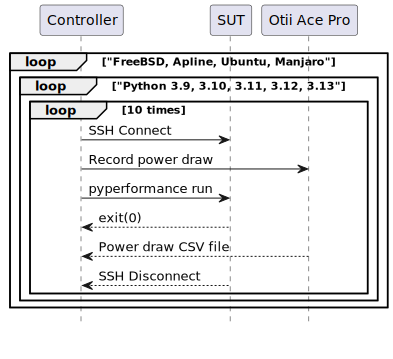
\includegraphics[width=0.5\textwidth]{images/scenario.pdf}
    \caption{High-level sequence diagram showing the sequence of actions involved in running the experiment}
    \label{fig:sequence}
\end{figure}\todo{Put this in one figure with experiment design}

\todo{@Helge: continue here}
Per configuration of \gls{cpu}, \gls{os}, and version of \python, we execute the \gls{pyperformance} benchmarks ten times\todo{@oskar: you experiment script does it 11 times, why?}, see \autoref{fig:sequence}.




Note, \gls{pyperformance} is configured to execute each benchmark ten times\todo{Double check that! I believe it is more often.}


\autoref{fig:sequence} shows the actions involved in running the experiment, and how the three main devices interact with each other.
On each RPi, the process shown is repeated ten times for each unique combination of Python version, OS, and RPi, totalling 400 recordings across 40 configurations.
For detailed instructions on how to run the experiment, install the OSs and Pyperformance, open SSH sessions, and query temperature, see the repository.



\bibliographystyle{splncs04}
\bibliography{bibliography}
%



\end{document}
